The challenges for integrating Ontology into program analysis exist in
each of the four main steps: the design of an ontology for the domain,
the generation of the knowledge, the utilization of the knowledge
base, and the design of the entire framework.  In this section, we
discuss each of the challenges and present some principles we use to
address them. At the end, we describe PATO, 
the prototype framework we have developed to do ontology-based program
analysis.  % that we have developed in this work.

\subsection{Ontology Design}

\vspace*{.1in}\noindent {\bf Challenges} To create an ontology for any
domain, the first primary task is to define the vocabulary to be used
in the domain. That includes the definition of the concepts,
properties, and restrictions in the domain.
These definitions establish the conceptual
terms and their relations of the ontology-based knowledge base for the domain.
Even though there are some de facto procedures on
designing an ontology~\cite{noy2001ontology}, program analysis has
some special challenges. %Unlike some other domains that has only
%several predefined kinds of tasks (e.g., navigation of a robot),
Program analysis has a large variety of tasks (e.g., loop analysis,
data access pattern analysis, alias analysis, dependence analysis,
liveness analysis, busy expression analysis, etc.) involving a huge
set of diverse concepts and relations.  Even a larger variety exists
in the input programs.  So the first question to use Ontology for
program analysis is how to design an intuitive, efficient and flexible
ontology that can facilitate the various program analyses and input
programs.

\vspace*{.1in}\noindent {\bf Solutions} 
Through our explorations, we have found the following three principles
helpful.

%\begin{itemize}
%\item
{\em Language standard-oriented design.}  When designing the
vocabulary of an ontology, it helps if one starts with reusing
language constructs and their categorizations defined in the standard
of the programming language of the target programs. Despite the
variety of the input programs, they are all artifacts following the
particular programming language. With the constructs and their
categorizations of the programming language covered, we can easily
express programs using the language in the ontology-based knowledge
base. This approach helps achieve a good coverage of the input
programs with familiar vocabulary for users.  For example, to model C
programs in an ontology, we followed the standard of C99 and enumerate
all program constructs and concepts in a top-down
fashion. Figure~\ref{fig:c_onto} shows a fraction of the top-level
ontology for C programs.  The main concepts in the domain include
variables, expressions, statements, and so on. The ``construct'' on the
edges indicate these vocabularies are the basic constructs in the C program domain.

%Examples of concepts include
%types, linkage of identifiers, name spaces of identifier, and so
%forth. 
\begin{figure}[h]
	\centering
	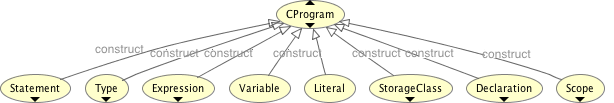
\includegraphics[width=\columnwidth]{graph/c_onto}	
	\caption{Top-level ontology for C program analysis.
		%\TODO{}
		}
	\label{fig:c_onto}
\end{figure}

%\item
{\em Being generic in property designs.}  Besides classes of concepts,
an ontology also contains a vocabulary for properties (or called
relations).  For example, an \textsf{Expression} instance may have
some \textsf{Type}, an \textsf{Identifier} may refer to some
\textsf{Definition}. Because there may be many properties to express,
in our practice, we follow a principle trying to define properties in
a generic way, and encode semantic meanings into concepts whenever
possible.  That allows the possible use of a small set of properties
and their combinations to express a large number of possible
properties in a program. For example, when describing \emph{an
  identifier has static storage class}, one approach is to define a
property \textsf{hasStaticStorage} and use it like \textsf{(someVar
  hasStaticStorage true)}.  Alternatively, we may define the concept
\textsf{Storage} as a class and use a simpler property
\textsf{hasStorage} as \textsf{(someVar hasStorage static)}, where
\textsf{static} is a member of \textsf{Storage}.  There are several
benefits for this second choice. First, using generic properties makes
the set of property vocabularies small and thus easy to manage.  For
example, \textsf{hasStorage} is used to describe all storage classes
instead of creating specific properties for each storage class.
Second, stripping semantics from property make writing logic rules
more flexible.  For example, the knowledge of \textsf{(someVar
  hasStorage static)} can be queried by the keyword
\textsf{hasStorage}.  Otherwise, users may need to use many specific
keywords as \textsf{hasStaticStorage}, \textsf{hasExternStorage}, and
so on.

%\item
{\em Continuous enrichment.}  In our exploration, we find that
continuous enrichment of the ontology vocabulary can be helpful. For
instance, in a canonical loop analysis, a user gives the description
of the concept of a canonical loop.  If that concept turns out to be
needed frequently (by many users), the concept could then be
integrated into the ontology framework to save the need for repeated
descriptions. Given that the program analysis ontology is intended to
be used by a community, a complexity is that different users may use
different names for a single user-defined relation (e.g., canonical
loop), making the detection of the repeated use of a user-level
concept difficult. Ontology-based logic reasoners come in handy. As the
descriptions of user-defined relations all use the vocabulary in the
same ontology, the reasoners can easily do a logic reasoning on the
descriptions to decide whether two user-defined relations are
equivalent. After recognizing the frequently needed user-level
concepts, such concepts can be added into the standard ontology for
future reuse.  
%Another benefit of such a feature is to support program
%analysis that requires some additional concepts that are not covered
%by existing vocabulary.
%\end{itemize}

Based on the three principles, we came up with an Ontology for C
program analysis, containing 178 concepts and 68 properties. It is not intended to be complete, but is sufficient for
examining the support of a single ontology to multiple different
program analyses as we will show later in this paper. 

\subsection{Knowledge Generation} % Knowledge Base Construction 

\vspace*{.1in}\noindent {\bf Challenges} 
Building up a knowledge base is essential for any application of
Ontology. For program analysis, the knowledge base shall include the
important knowledge related with the to-be-analyzed program. There are
three main questions to answer.  {\em (1) Ontology converter.} How to
construct an ontology converter that can automatically convert a given
program into the Ontology representation needed by many common program
analyses.  {\em (2) Naming.}  A program may contain functions,
statements, expressions, variables, and so on.  Any of them may appear
many times in difference locations. A challenge is what naming scheme
the ontology should use to reference each reference to avoid
ambiguity. {\em (3) Mapping.} One of the objectives of ontology-based
program analysis is to facilitate the cooperations among different
compilers and other program analysis tools. A difficulty is that they
may have different internal representations of a program.  To make
them able to interact based on the program ontology, the instances of
program constructs in the knowledge base should be possible to map to
some common ground meaningful to the different tools. One intuitive
choice of such common ground would be the source code of the
program. That will also make it easy for human to collaborate with
program analysis tools.  A complexity in using source code for
references is how to make the naming robust to code changes.  {\em (4)
  Space.} The knowledge about a program can be tremendous. Besides the
basic knowledge directly driven from the program, there could be many
other higher-level knowledge such as canonical loops, data dependences
among statements, and so on. This higher-level knowledge is derivable
from the lower-level knowledge. The derivation through reasoning may
take non-trivial time. But if all this knowledge is saved in the
knowledge base, the space cost could be large. How to strike a good
balance is important for practical usage of this new program analysis
paradigm.

\vspace*{.1in}\noindent {\bf Solutions} 
We come up with the following solutions to these
challenges. 

%\begin{itemize}
%\item
{\em Ontology converter.} Our experience shows that an ontology
converter can be easily created by building a translator on top of a
source-to-source compiler such as ROSE~\cite{ROSE}.  A
source-to-source compiler usually produces an abstract syntax tree
(AST) representation which is close to the input code. The translator
traverses the AST of the program to get structural and semantic
information, which is then stored into the knowledge base as
ontology. The program constructs are represented as individuals
(i.e. instances) of some of the classes defined in the language
ontology. Relations between them are represented by properties.
%The translator can be reused (with certain extensions) across programming languages as long as they use the same or similar form of AST. 

%\item
{\em Naming and Mapping.} 
In our naming scheme, we borrow the internationalized resource
identifiers (IRIs)~\cite{hitzler2009owl} that OWL uses. It helps avoid name conflicts. 
For the ontology of C program language, names of concepts are built directly from the corresponding terms used in the C language standard.
\footnote{We follow the naming convention of \textsf{UpperCamelCase}
  for classes and \textsf{lowerCamelCase} for properties.}  For
example, the concept \textsf{type} is referenced as \textsf{c:Type}.
An example IRI for the concept of types in a C program domain can look
like ``http://example.com/owl/CProgram:Type''.  Some alias can be
defined as short names for the prefix strings of a domain.
%We have an alias \textsf{c} for our C
%language domain. 

More care needs to be taken for designing the naming scheme for
representing the instances of a program construct.  Named constructs
such as types, variables, functions can use the C++ qualified name
concept to uniquely identify them.  For an unnamed construct (e.g. an
assignment statement) or a reference to named construct (e.g. variable
reference), a common intuitive approach is to use its location in the
source code of the program, such as $ \mathsf{file\ url,
  start\ location,end\ location} $ where the location is a pair of
(\textsf{line number}, \textsf{column number}). For instance,
``http://my.com/file1.c, 3:1, 5:1'' could refer to a loop that spans
from the beginning of the third line to the beginning of the fifth
line of file1.c. The problem with this scheme is that some minor
changes to the original program may invalidate all the names of the
constructs after the modification point.

We find {\em scoped IRI} useful to restrict the impact of a code
change to the names.  In {\em scoped IRI}, a name is composed of some
qualified names and some relative locations in the source code. For
constructs like functions, structures, global variables, we add their
scopes before their names. Other constructs within these constructs
are named by their locations, while the line numbers are relative to
the start line number of their surrounding constructs rather than the
beginning of the source-code file. Using this method, a global
variable declared in the first line of a file ``s.c'' (from column 5
to 6) can be named as \textsf{s.c::1:5,1:6}, while a variable declared
on the first line inside a function foo in file ``s.c'' (from column 6
to 10) can be named as \textsf{s.c::foo()::1:6,1:10}.  Thus, if there
is some change of the code, only the names in the same scope as the
changing point need to be updated.

%\item
{\em Space.} 
%Besides the basic knowledge on the program code,
%  there can be a lot of other relevant knowledge coming up in program
%  analysis. Due to the large variety of programs and relevant
%  analyses, saving all of them into the knowledge base could cause
%  space issues. 
To address the space challenge of putting everything into a knowledge
base, we split the knowledge base into a core knowledge base and
multiple loadable supplemental knowledge bases.  The core knowledge
base is always loaded and others are loaded as needed.  We also design
a cache-like management mechanism to alleviate the problem. It
maintains a buffer to store derived supplemental knowledge. When the
upper limit of the buffer gets reached, it starts to evict some of the
stored knowledge.
  %Here, the eviction
  %means removing the knowledge but keeping the commands for deriving
  %the knowledge such that when needed, the knowledge can be derived
  %quickly. 
  For the eviction policy, there can be multiple choices:
  least-recently-used (LRU), least-frequently-used (LFU), and their
  variants that are weighted with the size of the knowledge. 
  %We are
  %not aware of such solutions used in previous ontology-based systems
  %(in other domains).
%\end{itemize}

\subsection{Knowledge Utilization}

\vspace*{.1in}\noindent {\bf Challenges} Some challenges also exist in
the utilization of the knowledge base for program analysis.  {\em (1)
  Efficiency.}  In many cases (e.g., analyzing a large program), the
runtime efficiency of conducting a program analysis could be
important. A question to answer is whether the improved productivity
of the new paradigm hurts the runtime efficiency and if so, how to
improve the efficiency. {\em (2) Generality.}  Using descriptive
programming languages could be awkward for some usage cases,
especially when they involve some mathematical computations. Such
cases however do exist in some program analysis and optimizations, for
instance, when they relate with some performance models (an example is
the data placement optimizations Section~\ref{sec:exp} will
describe). Effectively overcoming such limitations is important for
the general applicability of ontology-based program analysis.

\vspace*{.1in}\noindent {\bf Solutions} We address these issues by
both creating some shortcuts and leveraging features of existing
ontology tools.

{\em Efficiency.}  Recent years have seen some significant improvement
of the performance of logic reasoners~\cite{tsarkov2006fact++, bassiliades2006defeasible}. 
%\TODO{cite some papers; see the related work section of some of Kemaphor's paper} 
  Many
optimizations have been developed.  For instance, in SWI-Prolog, the
ontology is stored as relation triples of \textsf{(subject property
  object)} with C extensions and some indices are built for each
element in the triples.  So a search of a particular element can be
done in constant time.  Additional optimizations can be applied to
queries.  For instance, Prolog provides the \emph{cut} operator (i.e.,
the ! symbol) to avoid unwanted backtracking in search. We find that
following some existing guidelines when writing
queries~\cite{Bratko2000} can be quite helpful for quickly
narrowing down the reasoner's search space.

In scenarios where the relevant knowledge base is simple and consists
of straightforward facts in triples (e.g., some memory
configurations), one may construct a customized lightweight parser in
high performance languages, which can further help achieve good
performance than going through a heavy-weight logic reasoner.

%\item
{\em Generality.} Ontology-based logic reasoning meets the needs of
many typical program analyses, but is not immediately natural for
expressing analyses that involve a lot of mathematical computations
(e.g., a regression-based performance modeling).  We find that a
mechanism called \emph{computable}~\cite{tenorth2009knowrob} in
Robotics can help resolve the issue. Computable is some special
ontology entity that can attach procedures to some classes or
properties.  When the deduction rule queries the individuals of one of
the classes or the properties, the associated procedures is invoked to
compute individuals for the target class or property. The procedure
can be written in a wide range of programming languages (e.g., C, C++,
Python).
%\end{itemize}

Besides allowing the direct input of queries by users written in logic
programming languages, ontology-based program analysis also allows
queries coming from a third-party software (which could be written in
even imperative languages like C, C++ or Java.) For such cases, the
ontology can be processed with libraries for those languages (e.g.,
the OWL API~\cite{horridge2011owl} or Prolog interface to foreign
languages\cite{bagnara2002foreign}). That offers the conveniences for
existing software tools (e.g., a compiler) to easily leverage a
program analysis ontology.


\subsection{Framework Design and PATO} 

The final challenge is how to organize the various components together
into a unified framework for program analysis. It includes choosing
the DL language and the reasoner that suit the needs of program
analysis, designing and implementing the APIs for both knowledge base
construction and queries, and integrating all the components together
into a complete cohesive framework that offers effective support to
various program analyses. 

\begin{figure}[ht]
\centering
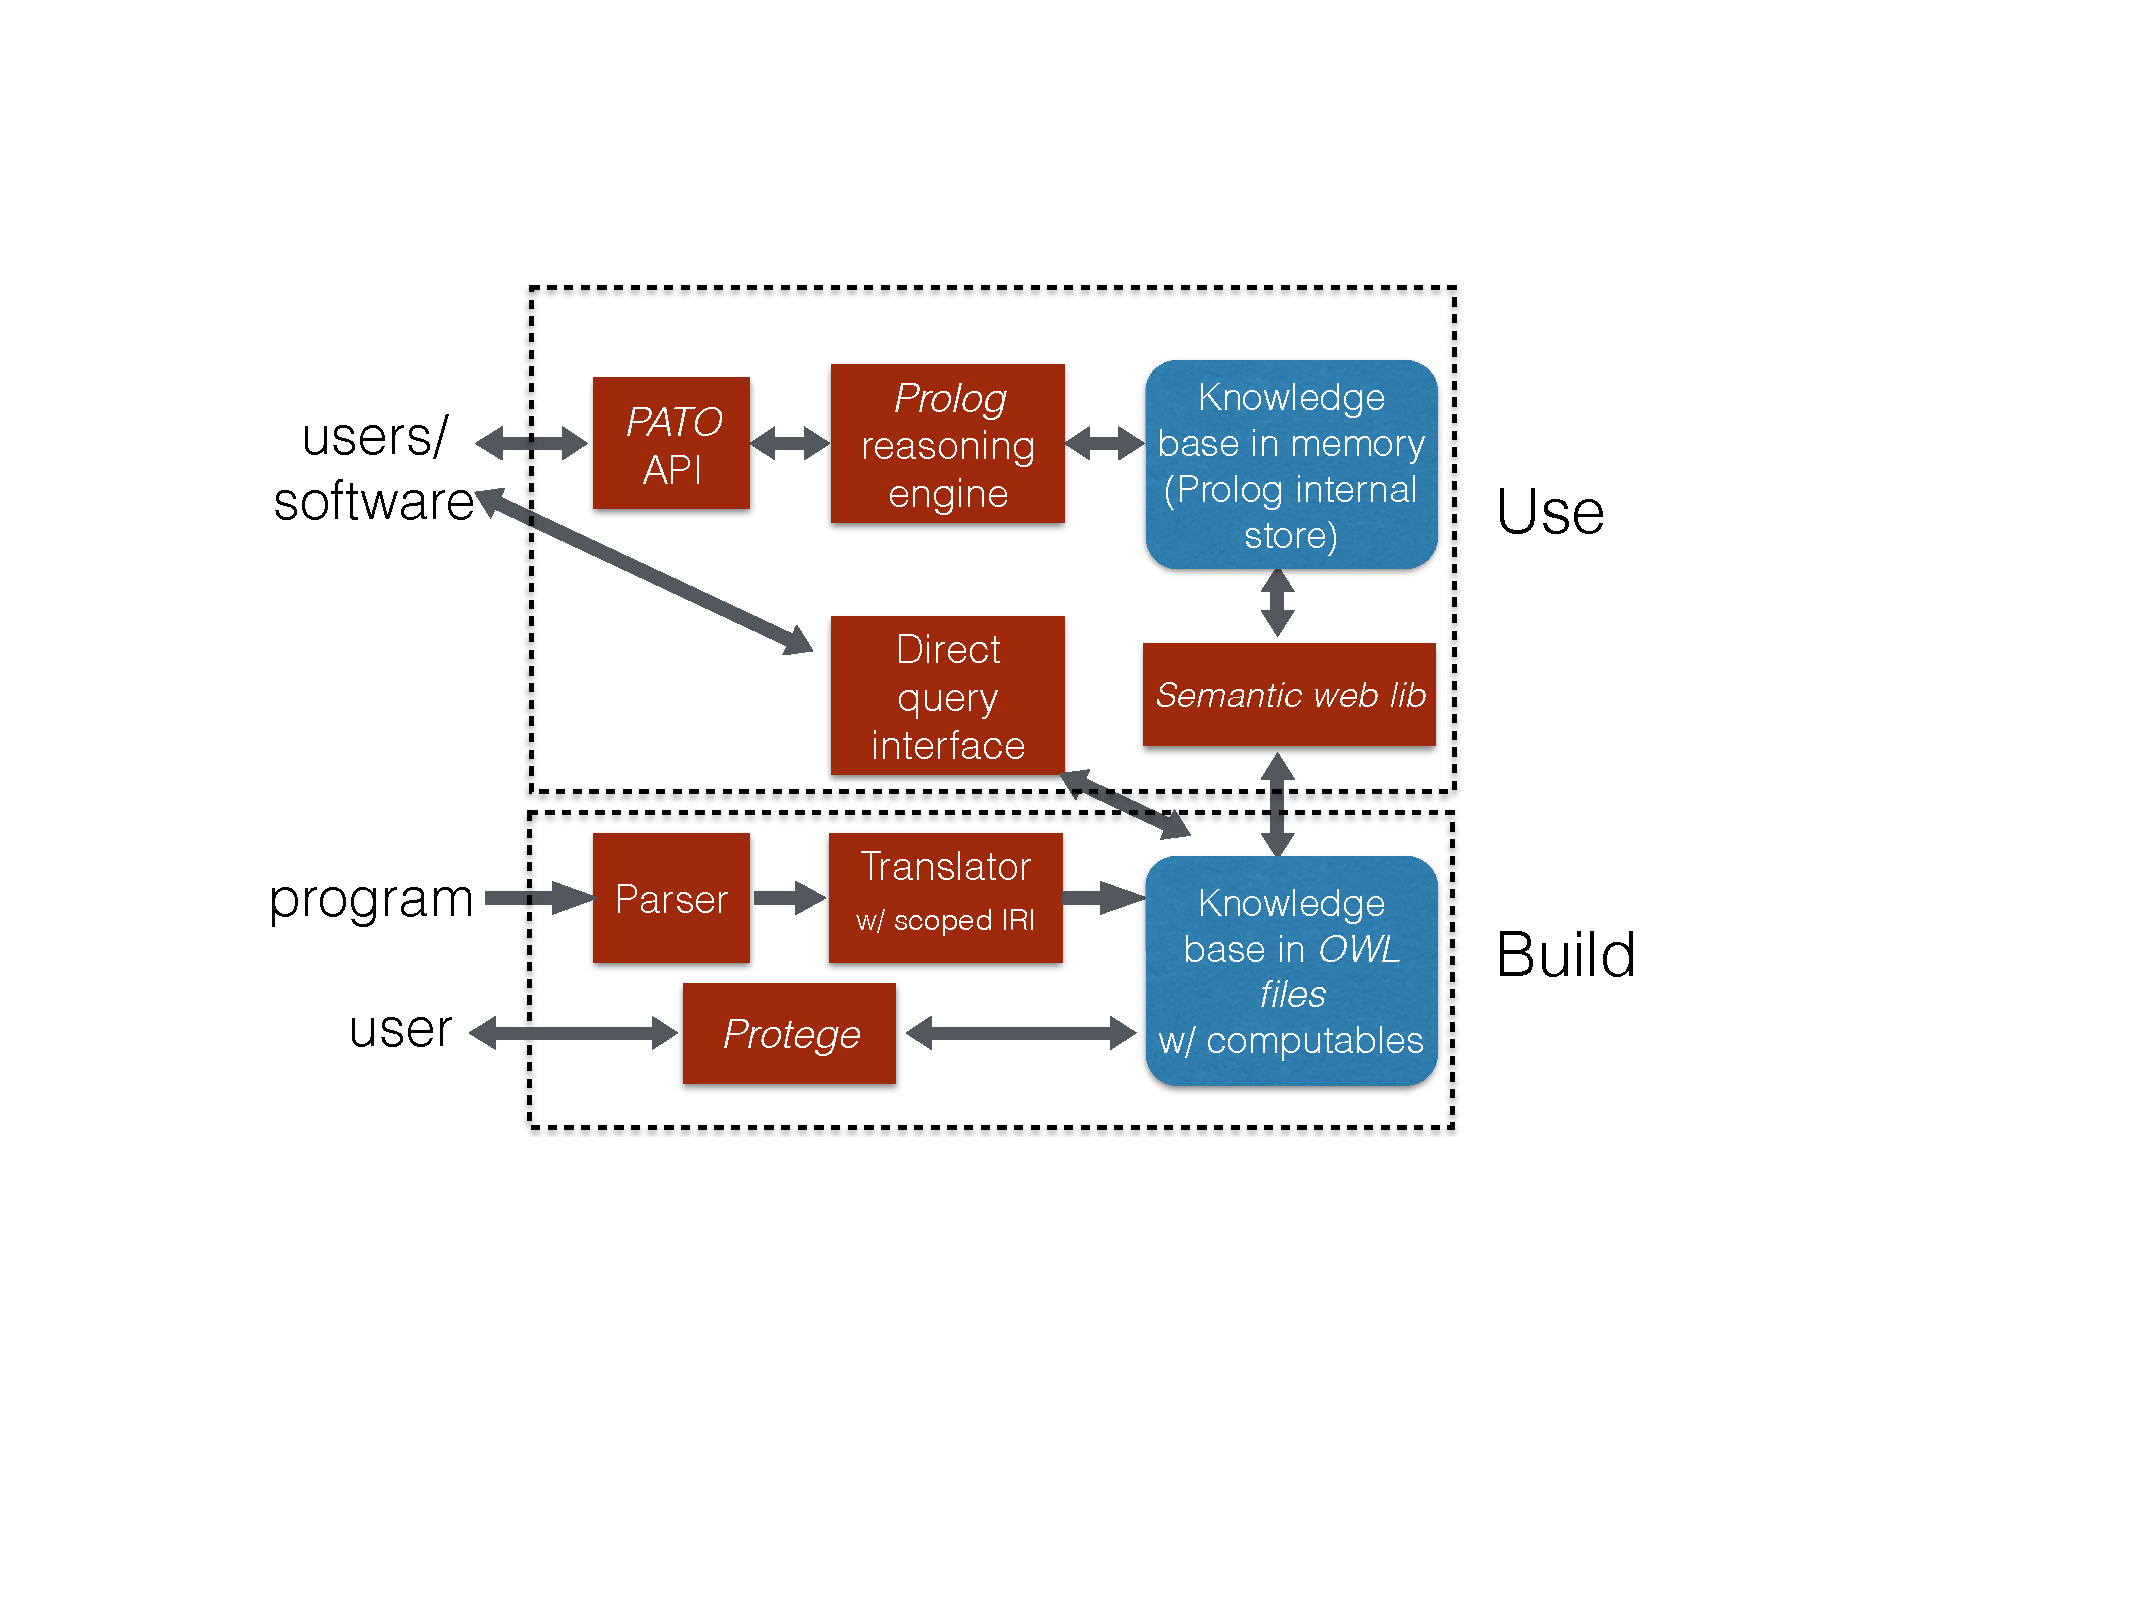
\includegraphics[width=.7\columnwidth]{graph/patoDiagram.pdf}
\caption{Structure of PATO.}
\label{fig:pato}
\end{figure}

To answer these questions, we have developed a prototype framework
named PATO for ontology-based program analysis. It integrates all the
aforementioned solutions to the various challenges, and leverages the
power of existing ontology tools.

Figure~\ref{fig:pato} outlines the main components of PATO. The
knowledge base in PATO can be in two forms, represented by the two
round-corner boxes on the right part of the figure. On the disk, the knowledge is stored as OWL files.
Each entry in the files is in an
OWL triple \textsf{(subject, property, object)}. For instance,
\textsf{(var1, hasValue, 0)} means a variable has a constant value of 0. The
reason for selecting this form is that OWL triple are
 one of the standard
(and space-efficient) formats for ontology representations and is
accepted by many Ontology tools. Another part of the knowledge base is
the {\em computables}, which are attached to the concepts and
properties in the triple collection. The cache-like buffering mechanism
is used to help with the space efficiency of the knowledge base.

Two of the primary ways to add knowledge into the knowledge base are
shown at the bottom of Figure~\ref{fig:pato}. In the first way, there
is a parser (based on ROSE~\cite{ROSE}) to convert an input program code into an AST preserving source level information. 
%The parser
%is currently only for C programs, but parsers for other languages can
%be easily plugged into the framework. 
We have also developed a translator
which translates the basic program knowledge on the AST into OWL 
triples and stores them into the knowledge base. During the
translation, the translator uses the scoped IRI (described in the
previous section) as the naming scheme. In the second way, we adopt
Stanford Protege~\cite{gennari2003evolution}, an interactive tool for ontology creation and manipulation.
Through its GUI, a user can intuitively add
entries into the knowledge base. The plugins of Protege
also provide many other features to the users, such as visualization, validation, and querying. 

There are two ways to use the knowledge base. In the first approach
(on top of Figure~\ref{fig:pato}), we incorporate the SWI-Prolog
reasoning engine. As the engine for a mature logic programming
language, it has been continuously enhanced in the last few decades in
efficiency, generality, and reliability. At the beginning of a usage,
the OWL files are loaded into memory, during which process, they are
converted into an internal knowledge base through the existing Semantic
Web Library. The in-memory organization of the
knowledge base features some efficient indexing schemes as mentioned
in the previous section and hence offers good efficiency.  When seeing
a query from a user or software agent, the Prolog engine would start
working on the internal knowledge base to provide the answers.  Prolog
provides a general interface for input logic rules and queries. We
have further developed a higher-level set of API tailored to represent
some common terms used in program analysis tasks (e.g., loops,
functions, etc.), through them, the users may write even more concise
descriptions.

The second approach to use the knowledge base is shown as the shortcut
(the diagonal path) in Figure~\ref{fig:pato}. Through a direct query
interface we have developed in C++, the user or software agent may
directly work on the OWL file collection (and computables) without
going through Prolog which may not be available to a user or too
costly to use in some special scenarios. For tasks which only need
some simple fact search (without the need for much reasoning), this
approach is more efficient than the Prolog-based approach because it
avoids the overhead in Prolog interpretation and other associated
cost.  Both the Prolog and the shortcut approach can insert new
knowledge (e.g., derived in a previous program analysis) into the
knowledge base.

%% The semantic web library provides a set of built-in rules for queries
%% like
%% \begin{itemize}
%% 	\item \emph{rdf(S, P, O)} returns the matching triple store.
%% 	\item \emph{rdf\_has(S, P, O)} considers the \emph{rdfs:subPropertyOf} relation of Predicate.
%% 	\item \emph{rdf\_reachable(S, P, O)} additionally follows the transitivity of predicate.
%% \end{itemize}
%% and our custom query rules are built upon these basic rules. For
%% example, the query rules in Listing~\ref{code:init}.

%% OpenK framework offers a rich set of the query rules as part of the
%% API for program analysis. Due to the modular design, new APIs are
%% added incrementally and easily. Although the query APIs are in Prolog
%% program, they can be used in C, C++, Java via the SWI-Prolog Foreign
%% Language Interface.

%user input via interface (file? interactive interface)

%% To represent the program construct individuals, we need to design a
%% portable and human readable ID first. A common approach is to use the
%% code location for source-level names. To accurately separate each
%% construct, we can name the ID in the form of
%% $$ \mathsf{start\ location,end\ location} $$ where the location is a
%% pair of (\textsf{line number}, \textsf{column number}).

%% % illustrate the ontology of program

%% The ontology of input code is built with the vocabularies defined in
%% the C program ontology. For example, when declaring membership of
%% constructs, the classes must be defined in the C ontology. Properties
%% of these constructs must be from the C ontology too. Here is a
%% fragment of C code

%% \begin{lstlisting}[numbersep=-8pt,firstnumber=0,caption=Example of ontology naming, label=code:id]
%% // s.c
%% int a = 0;
%% int foo() {
%%  for (int i = 0; i < 10; i++) {
%%   a = a + i;
%%  }
%% }
%% \end{lstlisting} 
%% and the snippet of ontology representation for the loop is
%% \begin{lstlisting}[caption=Ontology representation for the C snippet, label=code:onto_repr]
%% ('3:1,5:1', rdf:type, 'ForStatement')
%% ('3:6,3:14', rdf:type, 'VariableDecl')
%% ('3:6,3:10', rdf:type, Variable')
%% ('3:1,5:1', 'hasForInit', '3:6,3:14')
%% ('3:1,5:1', 'hasForTest', '3:17,3:22')
%% ('3:1,5:1', hasForIncr', '3:25,3:27')
%% ('3:1,5:1', hasBody', '3:30,5:1')
%% \end{lstlisting}

%% In the example, the \emph{for loop} is assigned with the id
%% \textsf{3:1,5:1}. It is described by the property as being a member of
%% the class \textsf{ForStatement}. It is also described as consisting
%% four components, namely, the declaration \textsf{int i = 0}, \textsf{i
%%   < 10}, \textsf{i++} and the for body. All of them are named with
%% their code location. This naming convention guarantees uniqueness and
%% also make it easy for human to locate the constructs.

%% However, if the original program is modified, all names of constructs
%% after the modification point must be updated. It is thus not portable,
%% especially when the ontology is used for code transformation. This
%% location-based naming method can be improved. Our solution is to use
%% qualified names and relative location-base names: for constructs like
%% functions, structures, global variables, we add their scopes before
%% their names. It is similar to the C++ qualified name. Other constructs
%% within these constructs are named by their location but the line
%% numbers are relative to the start line number of their surrounding
%% constructs. Using this method, the global variable \textsf{int a} in
%% Listing~\ref{code:id} is named as \textsf{s.c::1:5,1:6} and the variable
%% \textsf{int i} can be named as \textsf{s.c::foo()::1:6,1:10} (the
%% original is \textsf{3:6,3:10}). Thus, if there's some change of the
%% code, only small part of the code is needed to update.



